\documentclass[
  12pt,
  a4paper,
  parskip,
  openany
]{scrbook}

\usepackage[utf8]{inputenc}
\usepackage[english]{babel}

\usepackage[hidelinks, pdfusetitle]{hyperref}
\usepackage{enumitem}
\usepackage{suffix}
\usepackage{lipsum}
\usepackage{tabularx}

% Pandoc packages and options
\usepackage{longtable, booktabs}
\usepackage[T1]{fontenc}

\usepackage{lmodern}
\usepackage{textcomp}

\providecommand{\tightlist}{%
\setlength{\itemsep}{0pt}\setlength{\parskip}{0pt}}

% Citation packages and options
\usepackage{csquotes}
\usepackage[
  backend=biber,
  style=apa
]{biblatex}
\addbibresource{bibliography.bib}
\addbibresource{cassandra.bib}

% ===== INDIVIDUAL AUTHORS PER CHAPTER =====
% Source: https://tex.stackexchange.com/a/156865
\newcommand\chapterauthor[1]{\authortoc{#1}\printchapterauthor{#1}}
\WithSuffix\newcommand\chapterauthor*[1]{\printchapterauthor{#1}}

\makeatletter
\newcommand{\printchapterauthor}[1]{%
  {\parindent0pt\vspace*{-25pt}%
  \linespread{1.1}\large#1%
  \par\nobreak\vspace*{35pt}}
  \@afterheading%
}
\newcommand{\authortoc}[1]{%
  \addtocontents{toc}{\vskip-10pt}%
  \addtocontents{toc}{%
    \protect\contentsline{chapter}%
    {\hskip1.3em\mdseries\protect\scriptsize#1}{}{}}
  \addtocontents{toc}{\vskip5pt}%
}
\makeatother
% ==========================================


\title{NoSQL Databases}
\author{Daniel Rutz and Leon Schürmann (Eds.)}
\date{\today}

\begin{document}

\maketitle
\tableofcontents

\chapter{Apache Cassandra}
\chapterauthor{David Marchi, Daniel Schäfer, Erik Zeiske}

\section{Introduction}
%- History, relevance, environment, context
%- Task, goal, why, what
%- Structure
\subsection{Abstract}
\subsection{Overview of Cassandra}

\section{Wide Column Store}

\section{Use-Cases Cassandra is (not) suited for}  % I don't like this title

\section{Data Modelling}  % How to model data (or rather tables)

\section{Using the Cassandra Query Language}  % How to use CQL
This section will give a short overview of how to interact with a Cassandra database using the Cassandra Query Language (CQL), which is mainly inspired by the Structured Query Language (SQL) \autocite{cqlAlexMeng, newInCQL3, cassandra3cqldocCreateKeystore}.

\subsection {Creating a keyspace}
This similarity start by looking into how the creation of a keyspace is performed:
\begin{verbatim}
/* Create a new keyspace in CQL */
CREATE KEYSPACE data WITH replication =
\{'class': 'SimpleStrategy', 'replication_factor': 3\};

/* Create a new database in SQL */
CREATE DATABASE data;
\end{verbatim}
Hereby the only difference is that instead of creating a Database a keyspace is created and it is possible to specify which replication parameters should be used. What these parameter meen and how they should be used is explained later in Section \ref{sec:CassandraClusterArchitecture} \autocite{cqlAlexMeng}.

\subsection{Creating a table}
After creating a keyspace a table has to be created in order to hold the data. As a database is always part of a keyspace it is either necessary to specify the keyspace in every query or to simple scope every subsequent query into a given keyspace by using the USE query \autocite{cassandra3cqldocUse}:
\begin{verbatim}
USE data;
\end{verbatim}

Using this keyspace a table can be created using the same syntax as in SQL \autocite{cqlAlexMeng, newInCQL3, cassandra3cqldocCreateTable}:
\begin{verbatim}
CREATE TABLE groups (
   group_name varchar,
   group_location varchar,
   added_date date,
   username varchar,
   PRIMARY KEY (...)
);
\end{verbatim}

Hereby the only difference is how the primary key can be specified:
\begin{figure}[ht]
    \centering
\begin{verbatim}
      partition key       clustering key  clustering key
       |       |                |            |
((groupname, group_location), added_date, username)
\end{verbatim}
    \caption{Parts of a primary key specification in CQL \autocite{cqlPrimaryKeyDefinition}}
    \label{fig:cassandra:primaryKeyDefinition}
\end{figure}
The first part of the definition will always be the partition key. If it is a compound of several columns they need to be marked by parenthesis separated by comma in order to state that they as a hole build the partition key. If necessary the primary key can be followed by several clustering keys. Keep in mind that the data will be ordered first by the first clustering key after that by the second and so on. This means that a order by has to first called on the first clustering key and the fine ordering can be done on the subsequent one. It will not be possible to only order by the second or other subsequent clustering keys when not ordering by the first \autocite{cqlPrimaryKeyDefinition, cassandra3cqldocCreateTable}.

\subsection{Interacting with data}
In order to manipulate cassandra only provides three possible methods \autocite{cassandra_paper}:
\begin{itemize}
    \item insert(table, key, rowMutation)
    \item get(table, key, columnName)
    \item delete(table, key, columnName)
\end{itemize}
All having in common that the whole primary key has to be specified in order to interact with the data. The only exception hereby is the getting of data where only the partition key has to be specified.

Important to note is that there is no interaction to update a data entry. The reason for that is that as Cassandra is optimized for high write throughput is is very costly to read any data before writing. This means that an update and insert known from SQL will perform the same action on the data \autocite{cqlAlexMeng, newInCQL3}:
\begin{verbatim}
/* Inserting Data */
INSERT INTO Person (lastname, name, email)
VALUES ('Musterfrau', 'Maxi', 'maxi@gmail.com');

/* Updating Data */
UPDATE Person SET email = 'maxi@gmail.com'
WHERE lastname='Musterfrau' AND name = 'MAXI';
\end{verbatim}

As getting and deleting data is also similar to SQL there is no need to go into it any further in this section \autocite{cqlAlexMeng, cassandra3cqldocSelect}:
\begin{verbatim}
/* Selecting Data */
SELECT * FROM Person
  WHERE lastname='Musterfrau' AND name = 'Maxi';
/* Deleting Data */
DELETE FROM Person
  WHERE lastname='Musterfrau' AND name = 'Maxi';
\end{verbatim}

\section{Local reads and writes}
In order to perform the requested changed to the data they have to be written into the database. This section will take a look into how the changes will be written on a single node not taken into account the cluster.

\begin{figure}[ht]
    \centering
    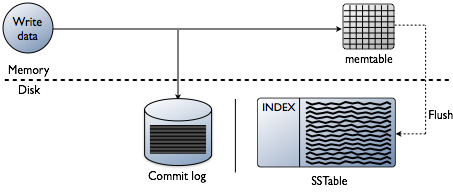
\includegraphics[width=0.75\textwidth]{img/cassandra_local_write.png}
    \caption{Writing data to Cassandra node \autocite{datastaxWriteData}}
    \label{fig:cassandra:writeData}
\end{figure}
In figure \ref{fig:cassandra:writeData} it can be seen that the write processe to cassadra involves three steps:
\begin{enumerate}
\item \textbf{Write to journal} Hereby the query is simple append to the journal on the disk, making it persistent even if the node goes down. As this action is a simple append it is very fast and leaves the data in a temporal order in the journal.
\item \textbf{Write to memtable} After writing to the journal the change is performed in the memtable putting the data into a Sorted String Table (SSTable). This form is the same form the data will be written on disk,
\item \textbf{Flush to disk when memtable is too big} This allows to simple flush the data and some metadata to the disk when it gets to big for the memory to hold it. Hereby a new data file is created not touching any of the previously written files, making this action also quite fast as no lookups have to be performed.
\end{enumerate}

After writing the data it also can be read again as shown by figure \ref{fig:cassandra:readData}:
\begin{figure}[ht]
    \centering
    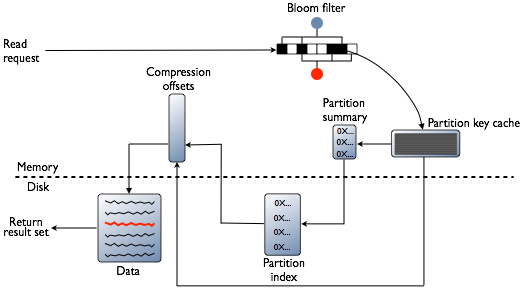
\includegraphics[width=0.75\textwidth]{img/cassandra_local_read.png}
    \caption{Reading data from Cassandra node \autocite{datastaxReadData}}
    \label{fig:cassandra:readData}
\end{figure}
\begin{enumerate}
    \item \textbf{Check caches} First the last query cache will be checked. Returning the data right away if it was requested in the near past.
    \item \textbf{Check memtable} Afterwards the memtable will be checked if it has recent activities on the requested data.
    \item \textbf{Find SSTable and location} If no entry was found in the memtable the data on disk will be checked by firstly determining in which memtable dump the dataset will be and then retriving it from there.
    \item \textbf{Merge with memtable} If it was necessary to retrieve the data from disk the data will be written to the memtable to allow later queries on the same data to succeed erlier.
\end{enumerate}

\section{Cluster Architecture}\label{sec:CassandraClusterArchitecture}  % How the cluster works

\section{Distributed writes and reads (CAP Theorem)}

\section{Setup and Configuration}  % Setup

\section{Summary and Conclusion}


\printbibliography

\end{document}
